% Created by tikzDevice version 0.12.3 on 2019-12-18 13:31:57
% !TEX encoding = UTF-8 Unicode
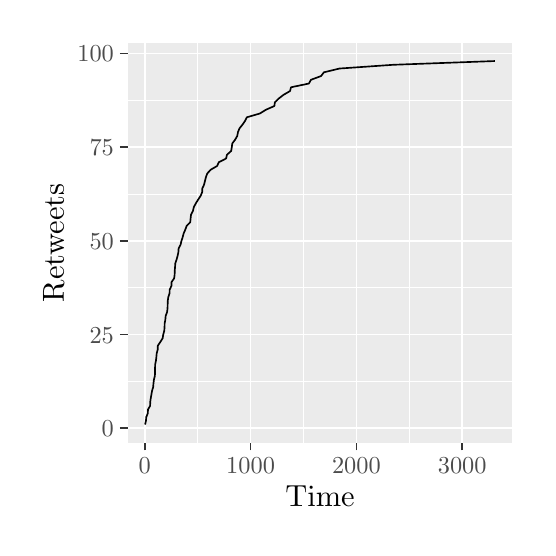
\begin{tikzpicture}[x=1pt,y=1pt]
\definecolor{fillColor}{RGB}{255,255,255}
\path[use as bounding box,fill=fillColor,fill opacity=0.00] (0,0) rectangle (180.67,180.67);
\begin{scope}
\path[clip] (  0.00,  0.00) rectangle (180.67,180.67);
\definecolor{drawColor}{RGB}{255,255,255}
\definecolor{fillColor}{RGB}{255,255,255}

\path[draw=drawColor,line width= 0.6pt,line join=round,line cap=round,fill=fillColor] (  0.00,  0.00) rectangle (180.68,180.68);
\end{scope}
\begin{scope}
\path[clip] ( 36.11, 30.69) rectangle (175.17,175.17);
\definecolor{fillColor}{gray}{0.92}

\path[fill=fillColor] ( 36.11, 30.69) rectangle (175.17,175.17);
\definecolor{drawColor}{RGB}{255,255,255}

\path[draw=drawColor,line width= 0.3pt,line join=round] ( 36.11, 52.83) --
	(175.17, 52.83);

\path[draw=drawColor,line width= 0.3pt,line join=round] ( 36.11, 86.68) --
	(175.17, 86.68);

\path[draw=drawColor,line width= 0.3pt,line join=round] ( 36.11,120.53) --
	(175.17,120.53);

\path[draw=drawColor,line width= 0.3pt,line join=round] ( 36.11,154.39) --
	(175.17,154.39);

\path[draw=drawColor,line width= 0.3pt,line join=round] ( 61.44, 30.69) --
	( 61.44,175.17);

\path[draw=drawColor,line width= 0.3pt,line join=round] ( 99.67, 30.69) --
	( 99.67,175.17);

\path[draw=drawColor,line width= 0.3pt,line join=round] (137.90, 30.69) --
	(137.90,175.17);

\path[draw=drawColor,line width= 0.6pt,line join=round] ( 36.11, 35.90) --
	(175.17, 35.90);

\path[draw=drawColor,line width= 0.6pt,line join=round] ( 36.11, 69.75) --
	(175.17, 69.75);

\path[draw=drawColor,line width= 0.6pt,line join=round] ( 36.11,103.61) --
	(175.17,103.61);

\path[draw=drawColor,line width= 0.6pt,line join=round] ( 36.11,137.46) --
	(175.17,137.46);

\path[draw=drawColor,line width= 0.6pt,line join=round] ( 36.11,171.32) --
	(175.17,171.32);

\path[draw=drawColor,line width= 0.6pt,line join=round] ( 42.32, 30.69) --
	( 42.32,175.17);

\path[draw=drawColor,line width= 0.6pt,line join=round] ( 80.55, 30.69) --
	( 80.55,175.17);

\path[draw=drawColor,line width= 0.6pt,line join=round] (118.78, 30.69) --
	(118.78,175.17);

\path[draw=drawColor,line width= 0.6pt,line join=round] (157.01, 30.69) --
	(157.01,175.17);
\definecolor{drawColor}{RGB}{0,0,0}

\path[draw=drawColor,line width= 0.6pt,line join=round] ( 42.43, 37.25) --
	( 42.75, 38.61) --
	( 42.85, 39.96) --
	( 43.42, 41.32) --
	( 43.47, 42.67) --
	( 44.25, 44.02) --
	( 44.28, 45.38) --
	( 44.47, 46.73) --
	( 44.71, 48.09) --
	( 44.94, 49.44) --
	( 45.35, 50.80) --
	( 45.45, 52.15) --
	( 45.63, 53.50) --
	( 45.97, 54.86) --
	( 46.01, 56.21) --
	( 46.03, 57.57) --
	( 46.05, 58.92) --
	( 46.34, 60.27) --
	( 46.50, 61.63) --
	( 46.62, 62.98) --
	( 46.99, 64.34) --
	( 47.00, 65.69) --
	( 47.89, 67.05) --
	( 48.77, 68.40) --
	( 48.98, 69.75) --
	( 49.35, 71.11) --
	( 49.46, 72.46) --
	( 49.50, 73.82) --
	( 49.75, 75.17) --
	( 49.86, 76.52) --
	( 50.37, 77.88) --
	( 50.54, 79.23) --
	( 50.58, 80.59) --
	( 50.62, 81.94) --
	( 50.82, 83.30) --
	( 51.27, 84.65) --
	( 51.31, 86.00) --
	( 51.95, 87.36) --
	( 51.97, 88.71) --
	( 52.92, 90.07) --
	( 53.11, 91.42) --
	( 53.13, 92.77) --
	( 53.25, 94.13) --
	( 53.34, 95.48) --
	( 53.80, 96.84) --
	( 54.17, 98.19) --
	( 54.46, 99.54) --
	( 54.54,100.90) --
	( 55.26,102.25) --
	( 55.55,103.61) --
	( 56.00,104.96) --
	( 56.36,106.32) --
	( 56.95,107.67) --
	( 57.44,109.02) --
	( 58.75,110.38) --
	( 58.87,111.73) --
	( 59.02,113.09) --
	( 59.73,114.44) --
	( 60.02,115.79) --
	( 60.74,117.15) --
	( 61.57,118.50) --
	( 62.47,119.86) --
	( 63.05,121.21) --
	( 63.11,122.57) --
	( 63.73,123.92) --
	( 64.07,125.27) --
	( 64.40,126.63) --
	( 64.89,127.98) --
	( 66.13,129.34) --
	( 68.46,130.69) --
	( 69.06,132.04) --
	( 71.71,133.40) --
	( 72.01,134.75) --
	( 73.53,136.11) --
	( 73.76,137.46) --
	( 73.93,138.82) --
	( 74.95,140.17) --
	( 75.72,141.52) --
	( 75.98,142.88) --
	( 76.51,144.23) --
	( 77.59,145.59) --
	( 78.54,146.94) --
	( 79.21,148.29) --
	( 83.89,149.65) --
	( 86.07,151.00) --
	( 89.15,152.36) --
	( 89.33,153.71) --
	( 90.72,155.07) --
	( 92.49,156.42) --
	( 94.81,157.77) --
	( 95.15,159.13) --
	(101.61,160.48) --
	(102.37,161.84) --
	(106.03,163.19) --
	(107.04,164.54) --
	(112.67,165.90) --
	(132.00,167.25) --
	(168.85,168.61);
\end{scope}
\begin{scope}
\path[clip] (  0.00,  0.00) rectangle (180.67,180.67);
\definecolor{drawColor}{gray}{0.30}

\node[text=drawColor,anchor=base east,inner sep=0pt, outer sep=0pt, scale=  0.88] at ( 31.16, 32.87) {0};

\node[text=drawColor,anchor=base east,inner sep=0pt, outer sep=0pt, scale=  0.88] at ( 31.16, 66.72) {25};

\node[text=drawColor,anchor=base east,inner sep=0pt, outer sep=0pt, scale=  0.88] at ( 31.16,100.58) {50};

\node[text=drawColor,anchor=base east,inner sep=0pt, outer sep=0pt, scale=  0.88] at ( 31.16,134.43) {75};

\node[text=drawColor,anchor=base east,inner sep=0pt, outer sep=0pt, scale=  0.88] at ( 31.16,168.29) {100};
\end{scope}
\begin{scope}
\path[clip] (  0.00,  0.00) rectangle (180.67,180.67);
\definecolor{drawColor}{gray}{0.20}

\path[draw=drawColor,line width= 0.6pt,line join=round] ( 33.36, 35.90) --
	( 36.11, 35.90);

\path[draw=drawColor,line width= 0.6pt,line join=round] ( 33.36, 69.75) --
	( 36.11, 69.75);

\path[draw=drawColor,line width= 0.6pt,line join=round] ( 33.36,103.61) --
	( 36.11,103.61);

\path[draw=drawColor,line width= 0.6pt,line join=round] ( 33.36,137.46) --
	( 36.11,137.46);

\path[draw=drawColor,line width= 0.6pt,line join=round] ( 33.36,171.32) --
	( 36.11,171.32);
\end{scope}
\begin{scope}
\path[clip] (  0.00,  0.00) rectangle (180.67,180.67);
\definecolor{drawColor}{gray}{0.20}

\path[draw=drawColor,line width= 0.6pt,line join=round] ( 42.32, 27.94) --
	( 42.32, 30.69);

\path[draw=drawColor,line width= 0.6pt,line join=round] ( 80.55, 27.94) --
	( 80.55, 30.69);

\path[draw=drawColor,line width= 0.6pt,line join=round] (118.78, 27.94) --
	(118.78, 30.69);

\path[draw=drawColor,line width= 0.6pt,line join=round] (157.01, 27.94) --
	(157.01, 30.69);
\end{scope}
\begin{scope}
\path[clip] (  0.00,  0.00) rectangle (180.67,180.67);
\definecolor{drawColor}{gray}{0.30}

\node[text=drawColor,anchor=base,inner sep=0pt, outer sep=0pt, scale=  0.88] at ( 42.32, 19.68) {0};

\node[text=drawColor,anchor=base,inner sep=0pt, outer sep=0pt, scale=  0.88] at ( 80.55, 19.68) {1000};

\node[text=drawColor,anchor=base,inner sep=0pt, outer sep=0pt, scale=  0.88] at (118.78, 19.68) {2000};

\node[text=drawColor,anchor=base,inner sep=0pt, outer sep=0pt, scale=  0.88] at (157.01, 19.68) {3000};
\end{scope}
\begin{scope}
\path[clip] (  0.00,  0.00) rectangle (180.67,180.67);
\definecolor{drawColor}{RGB}{0,0,0}

\node[text=drawColor,anchor=base,inner sep=0pt, outer sep=0pt, scale=  1.10] at (105.64,  7.64) {Time};
\end{scope}
\begin{scope}
\path[clip] (  0.00,  0.00) rectangle (180.67,180.67);
\definecolor{drawColor}{RGB}{0,0,0}

\node[text=drawColor,rotate= 90.00,anchor=base,inner sep=0pt, outer sep=0pt, scale=  1.10] at ( 13.08,102.93) {Retweets};
\end{scope}
\end{tikzpicture}
